%===============================================================================
% LaTeX sjabloon voor de bachelorproef toegepaste informatica aan HOGENT
% Meer info op https://github.com/HoGentTIN/latex-hogent-report
%===============================================================================

\documentclass[dutch,dit,thesis]{hogentreport}

% TODO:
% - If necessary, replace the option `dit`' with your own department!
%   Valid entries are dbo, dbt, dgz, dit, dlo, dog, dsa, soa
% - If you write your thesis in English (remark: only possible after getting
%   explicit approval!), remove the option "dutch," or replace with "english".

\usepackage{lipsum} % For blind text, can be removed after adding actual content

%% Pictures to include in the text can be put in the graphics/ folder
\graphicspath{{../graphics/}}

%% For source code highlighting, requires pygments to be installed
%% Compile with the -shell-escape flag!
%% \usepackage[chapter]{minted}
%% If you compile with the make_thesis.{bat,sh} script, use the following
%% import instead:
\usepackage[chapter,outputdir=../output]{minted}
\usemintedstyle{solarized-light}

%% Formatting for minted environments.
\setminted{%
    autogobble,
    frame=lines,
    breaklines,
    linenos,
    tabsize=4
}

%% Ensure the list of listings is in the table of contents
\renewcommand\listoflistingscaption{%
    \IfLanguageName{dutch}{Lijst van codefragmenten}{List of listings}
}
\renewcommand\listingscaption{%
    \IfLanguageName{dutch}{Codefragment}{Listing}
}
\renewcommand*\listoflistings{%
    \cleardoublepage\phantomsection\addcontentsline{toc}{chapter}{\listoflistingscaption}%
    \listof{listing}{\listoflistingscaption}%
}

% Other packages not already included can be imported here

%%---------- Document metadata -------------------------------------------------
% TODO: Replace this with your own information
\author{Ernst Aarden}
\supervisor{Dhr. F. Van Houte}
\cosupervisor{Mevr. S. Beeckman}
\title[Optionele ondertitel]%
    {Titel van de bachelorproef}
\academicyear{\advance\year by -1 \the\year--\advance\year by 1 \the\year}
\examperiod{1}
\degreesought{\IfLanguageName{dutch}{Professionele bachelor in de toegepaste informatica}{Bachelor of applied computer science}}
\partialthesis{false} %% To display 'in partial fulfilment'
%\institution{Internshipcompany BVBA.}

%% Add global exceptions to the hyphenation here
\hyphenation{back-slash}

%% The bibliography (style and settings are  found in hogentthesis.cls)
\addbibresource{bachproef.bib}            %% Bibliography file
\addbibresource{../voorstel/voorstel.bib} %% Bibliography research proposal
\defbibheading{bibempty}{}

%% Prevent empty pages for right-handed chapter starts in twoside mode
\renewcommand{\cleardoublepage}{\clearpage}

\renewcommand{\arraystretch}{1.2}

%% Content starts here.
\begin{document}

%---------- Front matter -------------------------------------------------------

\frontmatter

\hypersetup{pageanchor=false} %% Disable page numbering references
%% Render a Dutch outer title page if the main language is English
\IfLanguageName{english}{%
    %% If necessary, information can be changed here
    \degreesought{Professionele Bachelor toegepaste informatica}%
    \begin{otherlanguage}{dutch}%
       \maketitle%
    \end{otherlanguage}%
}{}

%% Generates title page content
\maketitle
\hypersetup{pageanchor=true}

%%=============================================================================
%% Voorwoord
%%=============================================================================

\chapter*{\IfLanguageName{dutch}{Woord vooraf}{Preface}}%
\label{ch:voorwoord}

%% TODO:
%% Het voorwoord is het enige deel van de bachelorproef waar je vanuit je
%% eigen standpunt (``ik-vorm'') mag schrijven. Je kan hier bv. motiveren
%% waarom jij het onderwerp wil bespreken.
%% Vergeet ook niet te bedanken wie je geholpen/gesteund/... heeft

\lipsum[1-2]
%%=============================================================================
%% Samenvatting
%%=============================================================================

% TODO: De "abstract" of samenvatting is een kernachtige (~ 1 blz. voor een
% thesis) synthese van het document.
%
% Een goede abstract biedt een kernachtig antwoord op volgende vragen:
%
% 1. Waarover gaat de bachelorproef?
% 2. Waarom heb je er over geschreven?
% 3. Hoe heb je het onderzoek uitgevoerd?
% 4. Wat waren de resultaten? Wat blijkt uit je onderzoek?
% 5. Wat betekenen je resultaten? Wat is de relevantie voor het werkveld?
%
% Daarom bestaat een abstract uit volgende componenten:
%
% - inleiding + kaderen thema
% - probleemstelling
% - (centrale) onderzoeksvraag
% - onderzoeksdoelstelling
% - methodologie
% - resultaten (beperk tot de belangrijkste, relevant voor de onderzoeksvraag)
% - conclusies, aanbevelingen, beperkingen
%
% LET OP! Een samenvatting is GEEN voorwoord!

%%---------- Nederlandse samenvatting -----------------------------------------
%
% TODO: Als je je bachelorproef in het Engels schrijft, moet je eerst een
% Nederlandse samenvatting invoegen. Haal daarvoor onderstaande code uit
% commentaar.
% Wie zijn bachelorproef in het Nederlands schrijft, kan dit negeren, de inhoud
% wordt niet in het document ingevoegd.

\IfLanguageName{english}{%
\selectlanguage{dutch}
\chapter*{Samenvatting}
\lipsum[1-4]
\selectlanguage{english}
}{}

%%---------- Samenvatting -----------------------------------------------------
% De samenvatting in de hoofdtaal van het document

\chapter*{\IfLanguageName{dutch}{Samenvatting}{Abstract}}

\lipsum[1-4]


%---------- Inhoud, lijst figuren, ... -----------------------------------------

\tableofcontents

% In a list of figures, the complete caption will be included. To prevent this,
% ALWAYS add a short description in the caption!
%
%  \caption[short description]{elaborate description}
%
% If you do, only the short description will be used in the list of figures

\listoffigures

% If you included tables and/or source code listings, uncomment the appropriate
% lines.
\listoftables

\listoflistings

% Als je een lijst van afkortingen of termen wil toevoegen, dan hoort die
% hier thuis. Gebruik bijvoorbeeld de ``glossaries'' package.
% https://www.overleaf.com/learn/latex/Glossaries

%---------- Kern ---------------------------------------------------------------

\mainmatter{}

% De eerste hoofdstukken van een bachelorproef zijn meestal een inleiding op
% het onderwerp, literatuurstudie en verantwoording methodologie.
% Aarzel niet om een meer beschrijvende titel aan deze hoofdstukken te geven of
% om bijvoorbeeld de inleiding en/of stand van zaken over meerdere hoofdstukken
% te verspreiden!

%%=============================================================================
%% Inleiding
%%=============================================================================

\chapter{\IfLanguageName{dutch}{Inleiding}{Introduction}}%
\label{ch:inleiding}

De inleiding moet de lezer net genoeg informatie verschaffen om het onderwerp te begrijpen en in te zien waarom de onderzoeksvraag de moeite waard is om te onderzoeken. In de inleiding ga je literatuurverwijzingen beperken, zodat de tekst vlot leesbaar blijft. Je kan de inleiding verder onderverdelen in secties als dit de tekst verduidelijkt. Zaken die aan bod kunnen komen in de inleiding~\autocite{Pollefliet2011}:

\begin{itemize}
  \item context, achtergrond
  \item afbakenen van het onderwerp
  \item verantwoording van het onderwerp, methodologie
  \item probleemstelling
  \item onderzoeksdoelstelling
  \item onderzoeksvraag
  \item \ldots
\end{itemize}

\section{\IfLanguageName{dutch}{Probleemstelling}{Problem Statement}}%
\label{sec:probleemstelling}

Uit je probleemstelling moet duidelijk zijn dat je onderzoek een meerwaarde heeft voor een concrete doelgroep. De doelgroep moet goed gedefinieerd en afgelijnd zijn. Doelgroepen als ``bedrijven,'' ``KMO's'', systeembeheerders, enz.~zijn nog te vaag. Als je een lijstje kan maken van de personen/organisaties die een meerwaarde zullen vinden in deze bachelorproef (dit is eigenlijk je steekproefkader), dan is dat een indicatie dat de doelgroep goed gedefinieerd is. Dit kan een enkel bedrijf zijn of zelfs één persoon (je co-promotor/opdrachtgever).

\section{\IfLanguageName{dutch}{Onderzoeksvraag}{Research question}}%
\label{sec:onderzoeksvraag}

Wees zo concreet mogelijk bij het formuleren van je onderzoeksvraag. Een onderzoeksvraag is trouwens iets waar nog niemand op dit moment een antwoord heeft (voor zover je kan nagaan). Het opzoeken van bestaande informatie (bv. ``welke tools bestaan er voor deze toepassing?'') is dus geen onderzoeksvraag. Je kan de onderzoeksvraag verder specifiëren in deelvragen. Bv.~als je onderzoek gaat over performantiemetingen, dan 

\section{\IfLanguageName{dutch}{Onderzoeksdoelstelling}{Research objective}}%
\label{sec:onderzoeksdoelstelling}

Wat is het beoogde resultaat van je bachelorproef? Wat zijn de criteria voor succes? Beschrijf die zo concreet mogelijk. Gaat het bv.\ om een proof-of-concept, een prototype, een verslag met aanbevelingen, een vergelijkende studie, enz.

\section{\IfLanguageName{dutch}{Opzet van deze bachelorproef}{Structure of this bachelor thesis}}%
\label{sec:opzet-bachelorproef}

% Het is gebruikelijk aan het einde van de inleiding een overzicht te
% geven van de opbouw van de rest van de tekst. Deze sectie bevat al een aanzet
% die je kan aanvullen/aanpassen in functie van je eigen tekst.

De rest van deze bachelorproef is als volgt opgebouwd:

In Hoofdstuk~\ref{ch:stand-van-zaken} wordt een overzicht gegeven van de stand van zaken binnen het onderzoeksdomein, op basis van een literatuurstudie.

In Hoofdstuk~\ref{ch:methodologie} wordt de methodologie toegelicht en worden de gebruikte onderzoekstechnieken besproken om een antwoord te kunnen formuleren op de onderzoeksvragen.

% TODO: Vul hier aan voor je eigen hoofstukken, één of twee zinnen per hoofdstuk

In Hoofdstuk~\ref{ch:conclusie}, tenslotte, wordt de conclusie gegeven en een antwoord geformuleerd op de onderzoeksvragen. Daarbij wordt ook een aanzet gegeven voor toekomstig onderzoek binnen dit domein.
\chapter{\IfLanguageName{dutch}{Stand van zaken}{State of the art}}%
\label{ch:stand-van-zaken}

% Tip: Begin elk hoofdstuk met een paragraaf inleiding die beschrijft hoe
% dit hoofdstuk past binnen het geheel van de bachelorproef. Geef in het
% bijzonder aan wat de link is met het vorige en volgende hoofdstuk.

% Pas na deze inleidende paragraaf komt de eerste sectiehoofding.

Dit hoofdstuk bevat je literatuurstudie. De inhoud gaat verder op de inleiding, maar zal het onderwerp van de bachelorproef *diepgaand* uitspitten. De bedoeling is dat de lezer na lezing van dit hoofdstuk helemaal op de hoogte is van de huidige stand van zaken (state-of-the-art) in het onderzoeksdomein. Iemand die niet vertrouwd is met het onderwerp, weet nu voldoende om de rest van het verhaal te kunnen volgen, zonder dat die er nog andere informatie moet over opzoeken \autocite{Pollefliet2011}.

Je verwijst bij elke bewering die je doet, vakterm die je introduceert, enz.\ naar je bronnen. In \LaTeX{} kan dat met het commando \texttt{$\backslash${textcite\{\}}} of \texttt{$\backslash${autocite\{\}}}. Als argument van het commando geef je de ``sleutel'' van een ``record'' in een bibliografische databank in het Bib\LaTeX{}-formaat (een tekstbestand). Als je expliciet naar de auteur verwijst in de zin (narratieve referentie), gebruik je \texttt{$\backslash${}textcite\{\}}. Soms is de auteursnaam niet expliciet een onderdeel van de zin, dan gebruik je \texttt{$\backslash${}autocite\{\}} (referentie tussen haakjes). Dit gebruik je bv.~bij een citaat, of om in het bijschrift van een overgenomen afbeelding, broncode, tabel, enz. te verwijzen naar de bron. In de volgende paragraaf een voorbeeld van elk.

\textcite{Knuth1998} schreef een van de standaardwerken over sorteer- en zoekalgoritmen. Experten zijn het erover eens dat cloud computing een interessante opportuniteit vormen, zowel voor gebruikers als voor dienstverleners op vlak van informatietechnologie~\autocite{Creeger2009}.

Let er ook op: het \texttt{cite}-commando voor de punt, dus binnen de zin. Je verwijst meteen naar een bron in de eerste zin die erop gebaseerd is, dus niet pas op het einde van een paragraaf.

\begin{figure}
  \centering
  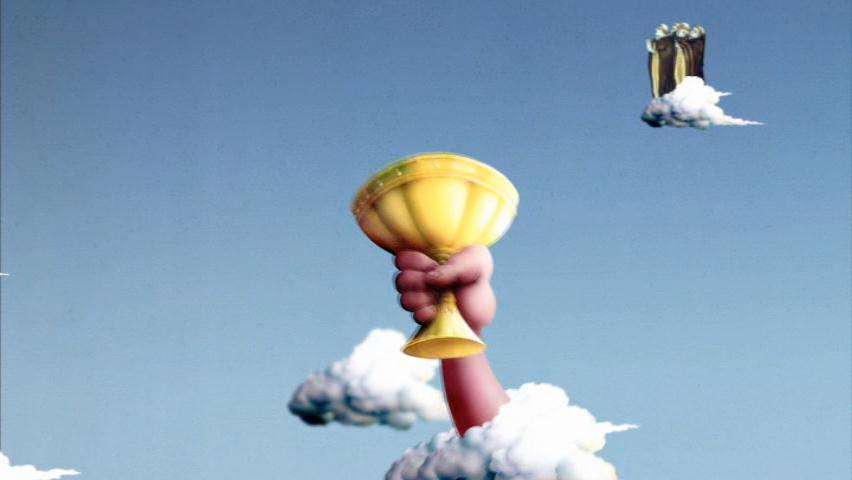
\includegraphics[width=0.8\textwidth]{grail.jpg}
  \caption[Voorbeeld figuur.]{\label{fig:grail}Voorbeeld van invoegen van een figuur. Zorg altijd voor een uitgebreid bijschrift dat de figuur volledig beschrijft zonder in de tekst te moeten gaan zoeken. Vergeet ook je bronvermelding niet!}
\end{figure}

\begin{listing}
  \begin{minted}{python}
    import pandas as pd
    import seaborn as sns

    penguins = sns.load_dataset('penguins')
    sns.relplot(data=penguins, x="flipper_length_mm", y="bill_length_mm", hue="species")
  \end{minted}
  \caption[Voorbeeld codefragment]{Voorbeeld van het invoegen van een codefragment.}
\end{listing}

\lipsum[7-20]

\begin{table}
  \centering
  \begin{tabular}{lcr}
    \toprule
    \textbf{Kolom 1} & \textbf{Kolom 2} & \textbf{Kolom 3} \\
    $\alpha$         & $\beta$          & $\gamma$         \\
    \midrule
    A                & 10.230           & a                \\
    B                & 45.678           & b                \\
    C                & 99.987           & c                \\
    \bottomrule
  \end{tabular}
  \caption[Voorbeeld tabel]{\label{tab:example}Voorbeeld van een tabel.}
\end{table}


%%=============================================================================
%% Methodologie
%%=============================================================================

\chapter{\IfLanguageName{dutch}{Methodologie}{Methodology}}%
\label{ch:methodologie}

%% TODO: In dit hoofstuk geef je een korte toelichting over hoe je te werk bent
%% gegaan. Verdeel je onderzoek in grote fasen, en licht in elke fase toe wat
%% de doelstelling was, welke deliverables daar uit gekomen zijn, en welke
%% onderzoeksmethoden je daarbij toegepast hebt. Verantwoord waarom je
%% op deze manier te werk gegaan bent.
%% 
%% Voorbeelden van zulke fasen zijn: literatuurstudie, opstellen van een
%% requirements-analyse, opstellen long-list (bij vergelijkende studie),
%% selectie van geschikte tools (bij vergelijkende studie, "short-list"),
%% opzetten testopstelling/PoC, uitvoeren testen en verzamelen
%% van resultaten, analyse van resultaten, ...
%%
%% !!!!! LET OP !!!!!
%%
%% Het is uitdrukkelijk NIET de bedoeling dat je het grootste deel van de corpus
%% van je bachelorproef in dit hoofstuk verwerkt! Dit hoofdstuk is eerder een
%% kort overzicht van je plan van aanpak.
%%
%% Maak voor elke fase (behalve het literatuuronderzoek) een NIEUW HOOFDSTUK aan
%% en geef het een gepaste titel.

\lipsum[21-25]



% Voeg hier je eigen hoofdstukken toe die de ``corpus'' van je bachelorproef
% vormen. De structuur en titels hangen af van je eigen onderzoek. Je kan bv.
% elke fase in je onderzoek in een apart hoofdstuk bespreken.

%\input{...}
%\input{...}
%...

%%=============================================================================
%% Conclusie
%%=============================================================================

\chapter{Conclusie}%
\label{ch:conclusie}

% TODO: Trek een duidelijke conclusie, in de vorm van een antwoord op de
% onderzoeksvra(a)g(en). Wat was jouw bijdrage aan het onderzoeksdomein en
% hoe biedt dit meerwaarde aan het vakgebied/doelgroep? 
% Reflecteer kritisch over het resultaat. In Engelse teksten wordt deze sectie
% ``Discussion'' genoemd. Had je deze uitkomst verwacht? Zijn er zaken die nog
% niet duidelijk zijn?
% Heeft het onderzoek geleid tot nieuwe vragen die uitnodigen tot verder 
%onderzoek?

\lipsum[76-80]



%---------- Bijlagen -----------------------------------------------------------

\appendix

\chapter{Onderzoeksvoorstel}

Het onderwerp van deze bachelorproef is gebaseerd op een onderzoeksvoorstel dat vooraf werd beoordeeld door de promotor. Dat voorstel is opgenomen in deze bijlage.

%% TODO: 
%\section*{Samenvatting}

% Kopieer en plak hier de samenvatting (abstract) van je onderzoeksvoorstel.

% Verwijzing naar het bestand met de inhoud van het onderzoeksvoorstel
%---------- Inleiding ---------------------------------------------------------

% TODO: Is dit voorstel gebaseerd op een paper van Research Methods die je
% vorig jaar hebt ingediend? Heb je daarbij eventueel samengewerkt met een
% andere student?
% Zo ja, haal dan de tekst hieronder uit commentaar en pas aan.

%\paragraph{Opmerking}

% Dit voorstel is gebaseerd op het onderzoeksvoorstel dat werd geschreven in het
% kader van het vak Research Methods dat ik (vorig/dit) academiejaar heb
% uitgewerkt (met medesturent VOORNAAM NAAM als mede-auteur).
% 

\section{Inleiding}%
\label{sec:inleiding}

Waarover zal je bachelorproef gaan? Introduceer het thema en zorg dat volgende zaken zeker duidelijk aanwezig zijn:

\begin{itemize}
  \item kaderen thema
  \item de doelgroep
  \item de probleemstelling en (centrale) onderzoeksvraag
  \item de onderzoeksdoelstelling
\end{itemize}

Denk er aan: een typische bachelorproef is \textit{toegepast onderzoek}, wat betekent dat je start vanuit een concrete probleemsituatie in bedrijfscontext, een \textbf{casus}. Het is belangrijk om je onderwerp goed af te bakenen: je gaat voor die \textit{ene specifieke probleemsituatie} op zoek naar een goede oplossing, op basis van de huidige kennis in het vakgebied.

De doelgroep moet ook concreet en duidelijk zijn, dus geen algemene of vaag gedefinieerde groepen zoals \emph{bedrijven}, \emph{developers}, \emph{Vlamingen}, enz. Je richt je in elk geval op it-professionals, een bachelorproef is geen populariserende tekst. Eén specifiek bedrijf (die te maken hebben met een concrete probleemsituatie) is dus beter dan \emph{bedrijven} in het algemeen.

Formuleer duidelijk de onderzoeksvraag! De begeleiders lezen nog steeds te veel voorstellen waarin we geen onderzoeksvraag terugvinden.

Schrijf ook iets over de doelstelling. Wat zie je als het concrete eindresultaat van je onderzoek, naast de uitgeschreven scriptie? Is het een proof-of-concept, een rapport met aanbevelingen, \ldots Met welk eindresultaat kan je je bachelorproef als een succes beschouwen?

%---------- Stand van zaken ---------------------------------------------------

\section{Literatuurstudie}%
\label{sec:literatuurstudie}
% Voor literatuurverwijzingen zijn er twee belangrijke commando's:
% \autocite{KEY} => (Auteur, jaartal) Gebruik dit als de naam van de auteur
%   geen onderdeel is van de zin.
% \textcite{KEY} => Auteur (jaartal)  Gebruik dit als de auteursnaam wel een
%   functie heeft in de zin (bv. ``Uit onderzoek door Doll & Hill (1954) bleek
%   ...'')

\subsection{Kleurenblindheid op Android}
Kleurenblindheid, waaronder protanopie, deuteranopie en tritanopie, ontstaat door defecten in de 
fotoreceptoren in het netvlies, waardoor het moeilijk wordt om kleuren correct waar te nemen \autocite{Salih2020}. 
Dit heeft invloed op de gebruikerservaring van mensen met deze aandoeningen, vooral in digitale omgevingen. 
Android biedt al verschillende apps die gebruikers helpen bij het herkennen van kleuren, bijvoorbeeld 
in wetenschappelijke toepassingen zoals titraties met fenolftaleïne. Volgens \textcite{Bandyopadhyay2017} verbeteren 
de apps niet alleen de precisie in laboratoriumresultaten, maar vergroten ze ook de algehele gebruikerservaring 
door visuele beperkingen te beperken. Daarnaast zijn er algoritmes zoals LMS Daltonization en LAB-correctie 
ontwikkeld, die de waarneming van kleuren verbeteren, wat vooral nuttig is in digitale en interactieve 
omgevingen \autocite{Baswaraju2020}. Dit toont aan hoe technologische innovaties de toegankelijkheid kunnen vergroten. 
Volgens \textcite{Crawford2024} is het naleven van de WCAG 2.1-normen essentieel voor het waarborgen van de 
toegankelijkheid van apps, zeker met de verplichtingen die zijn vastgelegd in de Europese Toegankelijkheidswet.
De implementatie van deze richtlijnen helpt ontwikkelaars bij het ontwerpen van apps die breder toegankelijk
zijn voor mensen met visuele beperkingen.
\subsection{Android SDK}
De Android Software Development Kit (SDK) biedt ontwikkelaars de nodige tools voor het bouwen 
van apps die niet alleen interactief en responsief zijn, maar ook rekening houden met 
de toegankelijkheid van gebruikers. Dit is van groot belang voor mensen met visuele beperkingen 
zoals kleurenblindheid. De SDK bevat verschillende componenten die essentieel zijn voor het 
ontwikkelen van apps die visueel aangepast kunnen worden aan de behoeften van de gebruiker, 
zoals UI-elementen, content providers en API-integraties. Volgens \textcite{Geeks2024} kunnen ontwikkelaars 
met de Android SDK gebruik maken van functies zoals TalkBack, een schermlezer die tekst hardop 
voorleest en het gemakkelijker maakt om door een app te navigeren voor visueel gehandicapte gebruikers. 
Dit vergroot de bruikbaarheid van apps, vooral voor mensen met kleurenblindheid. De juiste integratie 
van API's en interactieve elementen zijn essentieel voor het creëren van apps die toegankelijk zijn 
voor mensen met verschillende beperkingen. Door deze integratie kan de app zich aanpassen aan de 
visuele behoeften van de gebruiker, wat bijdraagt aan een inclusievere gebruikerservaring \autocite{Lee2011}.
\subsection{Android Toegankelijkheid}
Android biedt een breed scala aan functies die specifiek gericht zijn op het verbeteren van 
de toegankelijkheid van apps. Het is van groot belang dat ontwikkelaars deze functies vanaf de 
ontwerpfase meenemen, zodat de app geschikt is voor gebruikers met visuele beperkingen, zoals 
kleurenblindheid. Functies zoals inhoud beschrijvingen voor afbeeldingen, spraakcommando’s en de 
TalkBack-schermlezer dragen bij aan de bruikbaarheid van apps voor visueel gehandicapte 
gebruikers \autocite{Swearngin2024}. Door deze technologieën te integreren, kunnen ontwikkelaars de 
toegankelijkheid van apps aanzienlijk verbeteren en ervoor zorgen dat deze goed bruikbaar zijn voor 
mensen met verschillende vormen van kleurenblindheid. Het testen van de toegankelijkheid van apps 
tijdens de ontwerpfase is cruciaal, zoals recent onderzoek benadrukt \textcite{Gregorio2022}. Dit stelt 
ontwikkelaars in staat om de interactie van gebruikers met de app te optimaliseren en te zorgen voor 
een naadloze ervaring, ongeacht visuele beperkingen.



%---------- Methodologie ------------------------------------------------------
\section{Methodologie}%
\label{sec:methodologie}

Hier beschrijf je hoe je van plan bent het onderzoek te voeren. Welke onderzoekstechniek ga je toepassen om elk van je onderzoeksvragen te beantwoorden? Gebruik je hiervoor literatuurstudie, interviews met belanghebbenden (bv.~voor requirements-analyse), experimenten, simulaties, vergelijkende studie, risico-analyse, PoC, \ldots?

Valt je onderwerp onder één van de typische soorten bachelorproeven die besproken zijn in de lessen Research Methods (bv.\ vergelijkende studie of risico-analyse)? Zorg er dan ook voor dat we duidelijk de verschillende stappen terug vinden die we verwachten in dit soort onderzoek!

Vermijd onderzoekstechnieken die geen objectieve, meetbare resultaten kunnen opleveren. Enquêtes, bijvoorbeeld, zijn voor een bachelorproef informatica meestal \textbf{niet geschikt}. De antwoorden zijn eerder meningen dan feiten en in de praktijk blijkt het ook bijzonder moeilijk om voldoende respondenten te vinden. Studenten die een enquête willen voeren, hebben meestal ook geen goede definitie van de populatie, waardoor ook niet kan aangetoond worden dat eventuele resultaten representatief zijn.

Uit dit onderdeel moet duidelijk naar voor komen dat je bachelorproef ook technisch voldoen\-de diepgang zal bevatten. Het zou niet kloppen als een bachelorproef informatica ook door bv.\ een student marketing zou kunnen uitgevoerd worden.

Je beschrijft ook al welke tools (hardware, software, diensten, \ldots) je denkt hiervoor te gebruiken of te ontwikkelen.

Probeer ook een tijdschatting te maken. Hoe lang zal je met elke fase van je onderzoek bezig zijn en wat zijn de concrete \emph{deliverables} in elke fase?

%---------- Verwachte resultaten ----------------------------------------------
\section{Verwacht resultaat, conclusie}%
\label{sec:verwachte_resultaten}

Hier beschrijf je welke resultaten je verwacht. Als je metingen en simulaties uitvoert, kan je hier al mock-ups maken van de grafieken samen met de verwachte conclusies. Benoem zeker al je assen en de onderdelen van de grafiek die je gaat gebruiken. Dit zorgt ervoor dat je concreet weet welk soort data je moet verzamelen en hoe je die moet meten.

Wat heeft de doelgroep van je onderzoek aan het resultaat? Op welke manier zorgt jouw bachelorproef voor een meerwaarde?

Hier beschrijf je wat je verwacht uit je onderzoek, met de motivatie waarom. Het is \textbf{niet} erg indien uit je onderzoek andere resultaten en conclusies vloeien dan dat je hier beschrijft: het is dan juist interessant om te onderzoeken waarom jouw hypothesen niet overeenkomen met de resultaten.



%%---------- Andere bijlagen --------------------------------------------------
% TODO: Voeg hier eventuele andere bijlagen toe. Bv. als je deze BP voor de
% tweede keer indient, een overzicht van de verbeteringen t.o.v. het origineel.
%\input{...}

%%---------- Backmatter, referentielijst ---------------------------------------

\backmatter{}

\setlength\bibitemsep{2pt} %% Add Some space between the bibliograpy entries
\printbibliography[heading=bibintoc]

\end{document}
